\documentclass[tikz, border=10pt]{standalone}
\usepackage{tikz}
\usetikzlibrary{shapes.multipart, positioning, arrows.meta, calc}

\begin{document}
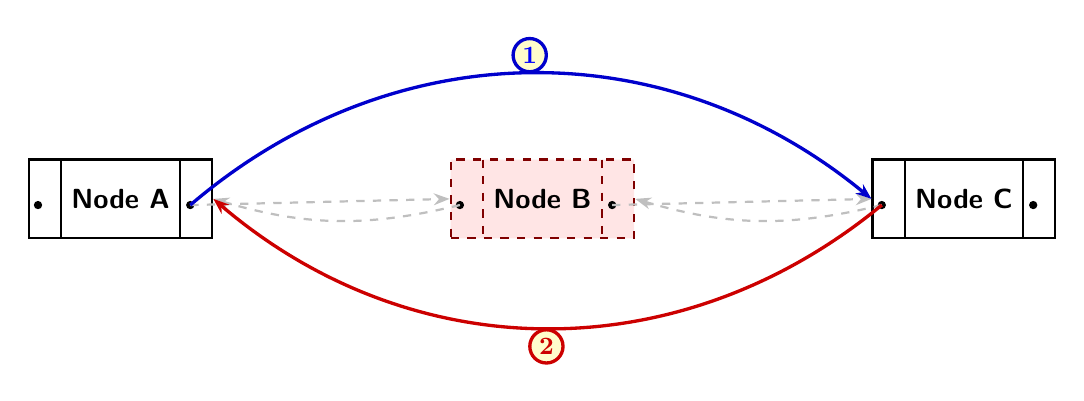
\begin{tikzpicture}[
    dblnode/.style={
        rectangle split,
        rectangle split parts=3,
        rectangle split horizontal,
        draw,
        thick,
        fill=white,
        minimum height=1cm,
        rectangle split part fill={white, white, white},
        font=\sffamily
    },
    delnode/.style={
        dblnode,
        fill=red!10,
        draw=red!50!black,
        dashed,
        rectangle split part fill={red!10, red!10, red!10}
    },
    ptr/.style={
        >={Stealth[length=2mm]},
        ->,
        thick,
        blue
    },
    revptr/.style={
        >={Stealth[length=2mm]},
        ->,
        thick,
        red!80!black
    },
    oldptr/.style={
        ptr,
        dashed,
        gray!50
    },
    oldrevptr/.style={
        revptr,
        dashed,
        gray!50
    },
    newptr/.style={
        ptr,
        draw=blue!80!black,
        very thick
    },
    newrevptr/.style={
        revptr,
        draw=red!80!black,
        very thick
    },
    stepmarker/.style={
        font=\small\bfseries,
        circle,
        draw,
        fill=yellow!20,
        inner sep=1pt,
        minimum size=12pt
    }
]

    % Nodes
    \node[dblnode] (nodeA) { \nodepart{one} \phantom{x} \nodepart{two} \textbf{Node A} \nodepart{three} \phantom{x}};
    \node[delnode, right=3cm of nodeA] (nodeB) { \nodepart{one} \phantom{x} \nodepart{two} \textbf{Node B} \nodepart{three} \phantom{x}};
    \node[dblnode, right=3cm of nodeB] (nodeC) { \nodepart{one} \phantom{x} \nodepart{two} \textbf{Node C} \nodepart{three} \phantom{x}};

    % Dots in pointer fields
    \fill[black] (nodeA.one) circle (1.5pt);
    \fill[black] (nodeA.three) circle (1.5pt);
    \fill[black] (nodeB.one) circle (1.5pt);
    \fill[black] (nodeB.three) circle (1.5pt);
    \fill[black] (nodeC.one) circle (1.5pt);
    \fill[black] (nodeC.three) circle (1.5pt);


    % Old links (A <-> B <-> C) - logical connections being removed/bypassed
    
    % A -> B
    \draw[oldptr] (nodeA.three) -- (nodeB.west);
    % B -> A
    \draw[oldrevptr] (nodeB.one) to[bend left=15] (nodeA.east);
    
    % B -> C
    \draw[oldptr] (nodeB.three) -- (nodeC.west);
    % C -> B
    \draw[oldrevptr] (nodeC.one) to[bend left=15] (nodeB.east);


    % New Pointers with steps
    
    % 1. A.next -> C
    % Bypassing B
    \draw[newptr] (nodeA.three) to[bend left=40] node[midway, above, stepmarker] {1} (nodeC.west);
    
    % 2. C.prev -> A
    % Bypassing B
    \draw[newrevptr] (nodeC.one) to[bend left=40] node[midway, below, stepmarker] {2} (nodeA.east);

    
\end{tikzpicture}
\end{document}
